\section{Design}
Conceptualizing a single ETL process as an entity of type \textit{Task}, that is, the ``extraction, transformation and loading of data from a source to destination'', provides a focal point on which the nETL software can be architected. Handling of instances of type \textit{Task} is done by an entity of type \textit{TaskManager}, which for the purposes of nETL v0.1 is implemented as a singleton (many instances of \textit{TaskManager} could potentially be useful if scaling of nETL were required). Objects of type \textit{Task} are instantiated via a \textit{Task} constructor, which takes a configuration object as an argument. This configuration is specified as a JSON file in which an operation of type \textit{Extraction}, operation(s) of type \textit{Transformation} and an operation of type \textit{Load} (E, T, and L operation objects) is described.

Starting the long-running nETL process comprises instantiation the singleton instance of type \textit{App}. This object holds references to the singleton instance of \textit{TaskManager} (taskManager), the E, T, and L operations and provides a CLI (command line interface) to facilitate user interactions. Via the CLI, users can interact with taskManager and load custom E, T, and L operations as well start/stop tasks, configure application options such as log output path, etc. Via the CLI, the taskManager object is also able to provide user-feedback on the progress of tasks, messages from the E, T, and L operations as well as display any program faults that may occur.

E, T, and L operations consist of JavaScript modules (JavaScript modules are executable functions) that should adhere to their respective contracts; specifically, the contracts stipulate an object return on invocation of the module that creates closure over a variety of functions that can then be invoked by taskManager according to the required operation specified by the task object.

\begin{figure}[H]
    \centering
    \begin{mdframed}
        \centering
        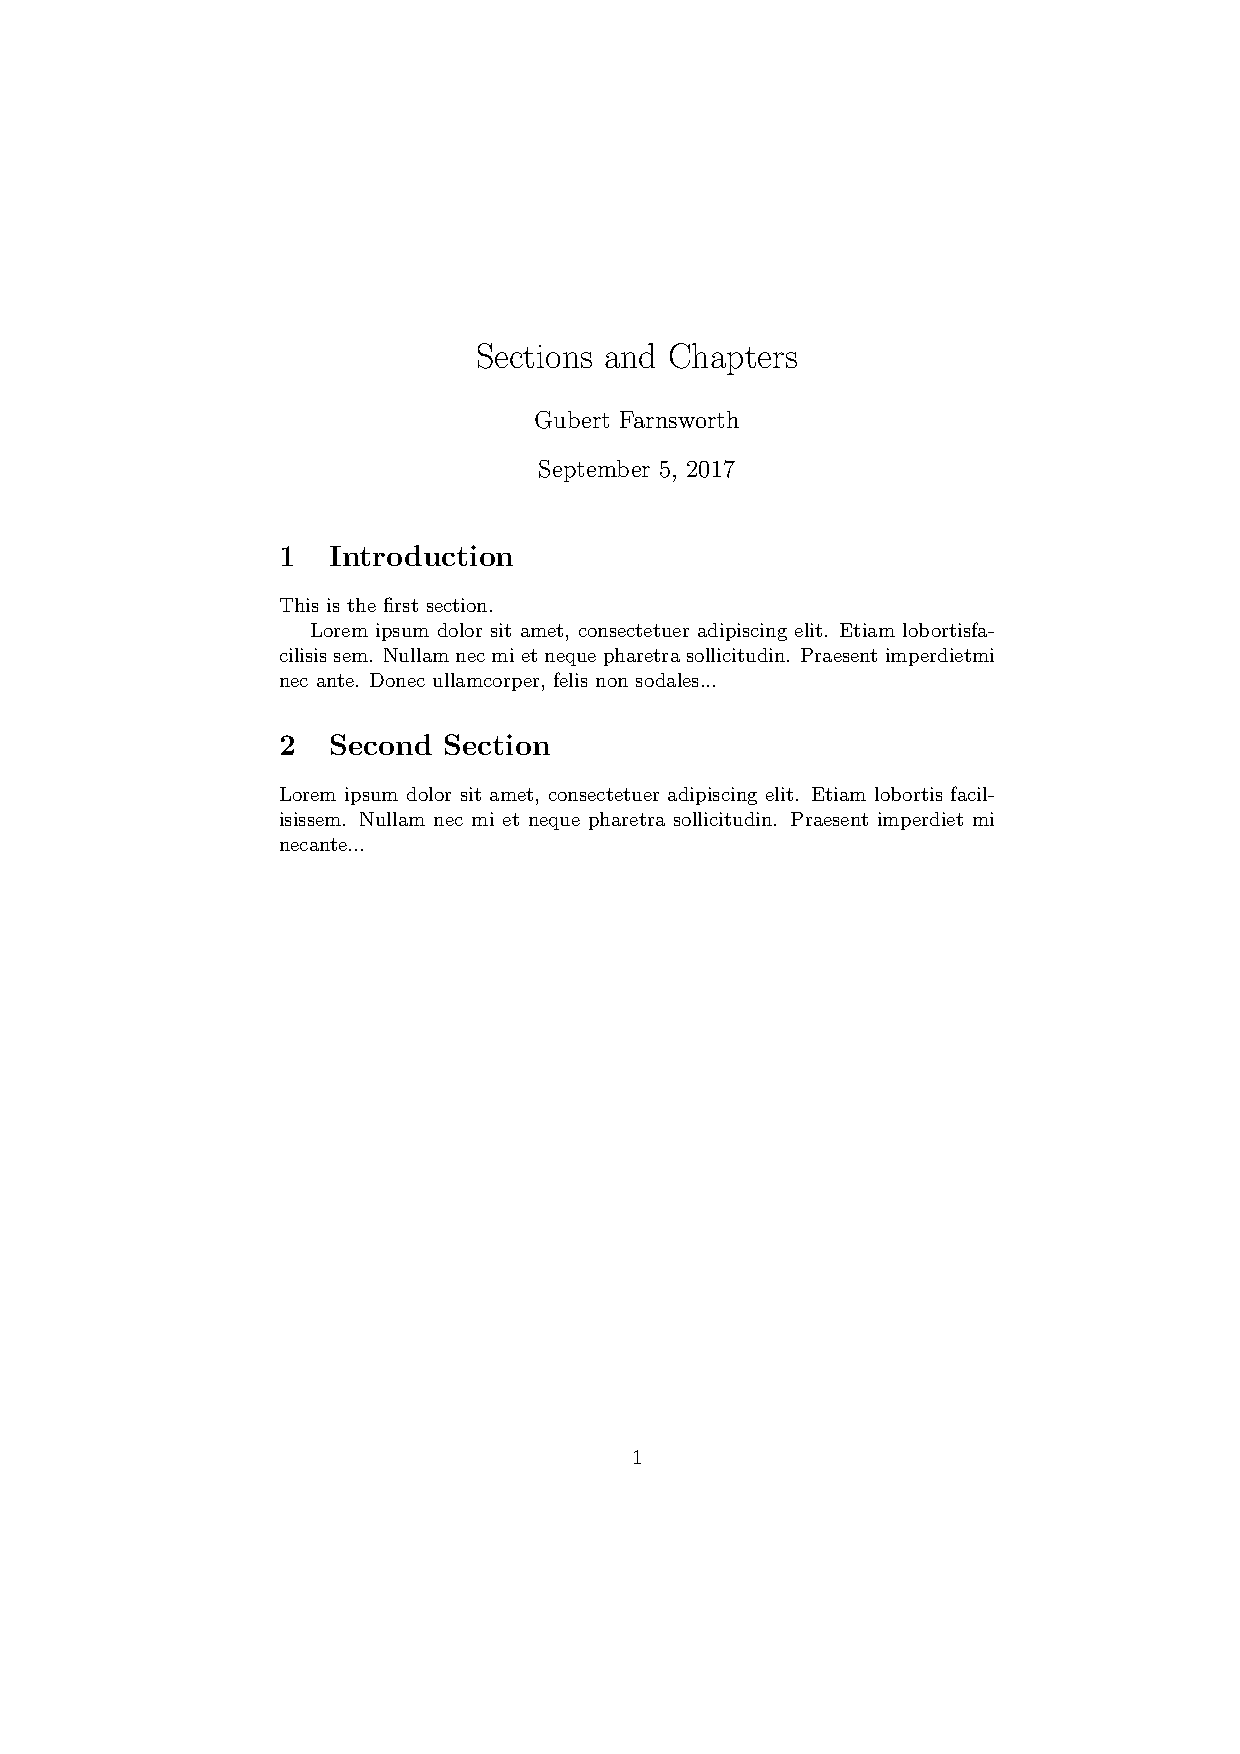
\includegraphics[scale=0.39]{./resources/figures/netl.png}
    \end{mdframed}
    \caption[nETL Architecture]{\textbf{Figure \ref{nETL}: nETL Architecture.} \textit{nETL} is an ETL framework designed to host user-created \textit{Modules} to define \textit{extraction}, \textit{transformation} and \textit{loading} processes. \textit{Modules}, shown in the colored boxes, consist of two parts: a configuration object (a JSON object) and a function that adheres to the specified contract. On startup the \textit{nETL} framework loads modules via the operations via a function made available by the main class. The modules are then cached in main memory by the \textit{nETL} process. A user can then interact with the TaskManager class to create a new task via loading a JSON configuration that makes use of a particular \textit{Module}. Tasks consist of an \textit{Extraction module} configuration, several \textit{Transformation module} configurations and a \textit{Load} configuration. Because modules are created and defined by users, as well as the order in which modules are executed, input/output contracts are also defined by the user, and as such \textit{ETL} processes are infinitely configurable.}
    \label{nETL}
\end{figure}

Figure \ref{nETL} shows a potential architecture for a configurable component-based ETL tool, including both the application framework and the E, T, and L operations components. JavaScript is a suitable language to prototype this application for a number of reasons:

\begin{itemize}
    \item It has a very succinct API making it fast to write code in (i.e. it is a highly abstracted language similarly to Ruby or Python)
    \item But unlike Ruby or Python (and other high level languages), it is opinionated in that it handles IO asynchronously by default
    \item The \textit{JavaScript} implementation of object-orientation is appealing (to some developers at least)
    \item And working and learning \textit{JavaScript} is very much in line with the spirit of CouchDB and the web in general
\end{itemize}

\subsection{Application Module}
The taskManager object is a simple JavaScript constructor, invoked once on app startup. The resultant object is reference by the main application and made available to the CLI user via closure as is typical when using the JavaScript module patterns. This patterns involves execution of a function and returning references to variables scoped within the function. Since these references remain after function execution the JavaScript garbage collector ignores them. But since they are scoped to the original function call they are private to the referenced return object (JavaScript-eque namespacing). An example of the Application module, instantiation of the taskManager singleton and the \textit{TaskManager} constructor itself is included in the appendix (see \ref{netl-application-module} and \ref{netl-taskmanager-constructor}).

Since IO in JavaScript is asynchronous, batching either needs to be run sequentially (batches are processed one after the other), or by carefully managing asynchronous execution of batches. Batches extracted asynchronously and concurrently would quickly overwhelm the network capabilities of any computer since thousands of network requests would be queued and most would fail. The easier way to handle state in this case (by far!) is serialize processing of batches. As such, nETL is implemented to execute tasks concurrently and asynchronously (not this is not truly parallel execution), and batches of data for a single task serially.

Such an implementation is achieved using JavaScript generators - a means of quickly implementing arbitrary iterators, including iterators over generated iterators \cite{mozillaGenerators} - as a means of serializing iterations over the data source. Once a user directs the application to run a task by the appropriate CLI command with the path to a task configuration specified as an argument, the taskManager object invokes a generator function to return an iterator over the specified data source via the specified \textit{Extraction} operation. This generator function is included in the appendix for reference (See \ref{netl-batch-generator}).

With batch generation serialized, processing each batch via specified E, T and L modules (as per task configuration) is straightforward; first the batch is iterated over, with all transformations applied sequentially to each item. Then the batch is loaded (at once) into the data destination as defined by the task configuration. Because the load operation is allowed to be asynchronous, it is necessary to await the result of the load operation before extracting the next batch. This is done via implementing extraction, transformation, load iteration recursively, with a callback passed to the Load module to re-execute the iterating function on a successful load (the callback is called on resolution of a JavaScript promise in this case). This recursive iterator is included in the appendix (see \ref{netl-recursive-iterator}). All the code snippets included are stripped down and don't include error handling or other code superfluous to the core logic.

\subsection{Extraction, Transformation, Load Modules}
On Module invocation, the contract for E, T, and L operations is that Module execution returns an object with two properties - ``name'': the identifier as used by the application engine to invoke the correct E, T, or L operations during task execution, and the property ``exe'': a pointer to the function that the application engine actually invokes. Closure over the ``exe'' and configuration properties mean that the modules are only evaluated once per task execution (a task may involve calling a transformation function millions of times - once for each item extracted from a CSV), so this is necessarily quite efficient. An example of code defining a module and loading that module into the application is included in the appendix (see \ref{netl-module-loading}).

A list of modules as written for, and used in this project is included in the appendix (see \ref{netl-modules}). Except for the FLATFILE extraction module, they consist of minimal amounts of code with simple logic. The FLATFILE module (see \ref{netl-extract-flatfile} in the appendix) uses a JavaScript generator as a means of serializing CSV line-extraction in regards to the rest of the ETL process. The generator creates an iterator over CSV file content as specified by an open source library available on Github \cite{bower16}.

The most important transformation applied to extracted CSV lines - i.e. the conversion of tabular data into objects uses the TEXT\_LINE\_TO\_OBJ Module (see \ref{netl-trans-text-line-to-obj} in the Appendix). This module makes use of a free CSV parsing library \cite{csvParse} to handle the intricately complex (and necessarily variable) process of properly delimiting CSV content.

nETL allows for configurable transformations to be applied to each extracted entity-object. Specifically, every object needs the property `type\_' appended to it. The CREATE\_OBJ\_FIELD \textit{nETL} module was composed for this task, the code of which is available in the appendix (\ref{netl-trans-create-obj-field}). Aside from appending additional properties to objects, transformation modules were written for filtering entire objects via whitelisting and filtering object properties via whitelisting.

The FILTER module allows users to configure a list of keys, and for each key, a list of values that objects are whitelisted on. The code for this module is available in the appendix at \ref{netl-trans-filter}. Distinct from the FILTER module is the WHITELIST module, as shown in the appendix at \ref{netl-trans-whitelist}. This module allows users to configure a list of keys that are whitelisted per object. (Modules are named according to the operation performed PER object; so the FILTER module filters entire objects, and the WHITELIST module filters properties of an object).

Loading data to CouchDB involves a straight forward network request. On the request response a callback as passed to the module is executed to continue the ETL iteration. Due to the cleaner API, Load modules are specifically required to return a promise as part of their contract. The Load Module as used to load data into CouchDB for this project is shown in the appendix (see \ref{netl-load-couchdb}). Network requests make use of the well-known, open-source node.js library ``request'' \cite{request-lib}.